\documentclass[border=6pt]{standalone}
\usepackage{listings}
\usepackage{xcolor}
\usepackage{tikz}
\usetikzlibrary{calc,backgrounds}

% ---------- Farben ----------
\definecolor{codebg}{RGB}{250,250,248}
\definecolor{codekw}{RGB}{60,90,190}       % normale Keywords
\definecolor{codecomment}{RGB}{140,140,140}
\definecolor{codestring}{RGB}{170,90,20}
\definecolor{newcol}{RGB}{40,140,90}       % NEU (grün)

\lstdefinelanguage{CUDAdiff}{
    language=C++,
    morekeywords=[1]{__global__, __device__, __host__, auto, static_cast,
    uint8_t, int32_t, uint32_t, constexpr},
    morekeywords=[2]{__constant__, __shared__, tile, tile_idx, tile_size,
    tx, ty, img_x, img_y, __syncthreads, BLOCK_SIZE, BLUR_RADIUS, device_weights},
}

\lstset{
    language=CUDAdiff,
    basicstyle=\ttfamily\small,
    keywordstyle=[1]\color{codekw}\bfseries,
    keywordstyle=[2]\color{newcol}\bfseries,
    commentstyle=\color{codecomment}\itshape,
    stringstyle=\color{codestring},
    numbers=left,
    numberstyle=\tiny\color{black!40},
    numbersep=6pt,
    frame=none,
    breaklines=true,
    breakautoindent=true,
    breakindent=1.5em,
    tabsize=2,
    showstringspaces=false,
    columns=flexible,
    xleftmargin=1.1em,
    framexleftmargin=1.1em,
    escapeinside={(@}{@)},
}

\newcommand{\tikzmark}[1]{\tikz[remember picture, overlay] \node[inner sep=0pt] (#1) {};}

\begin{document}
    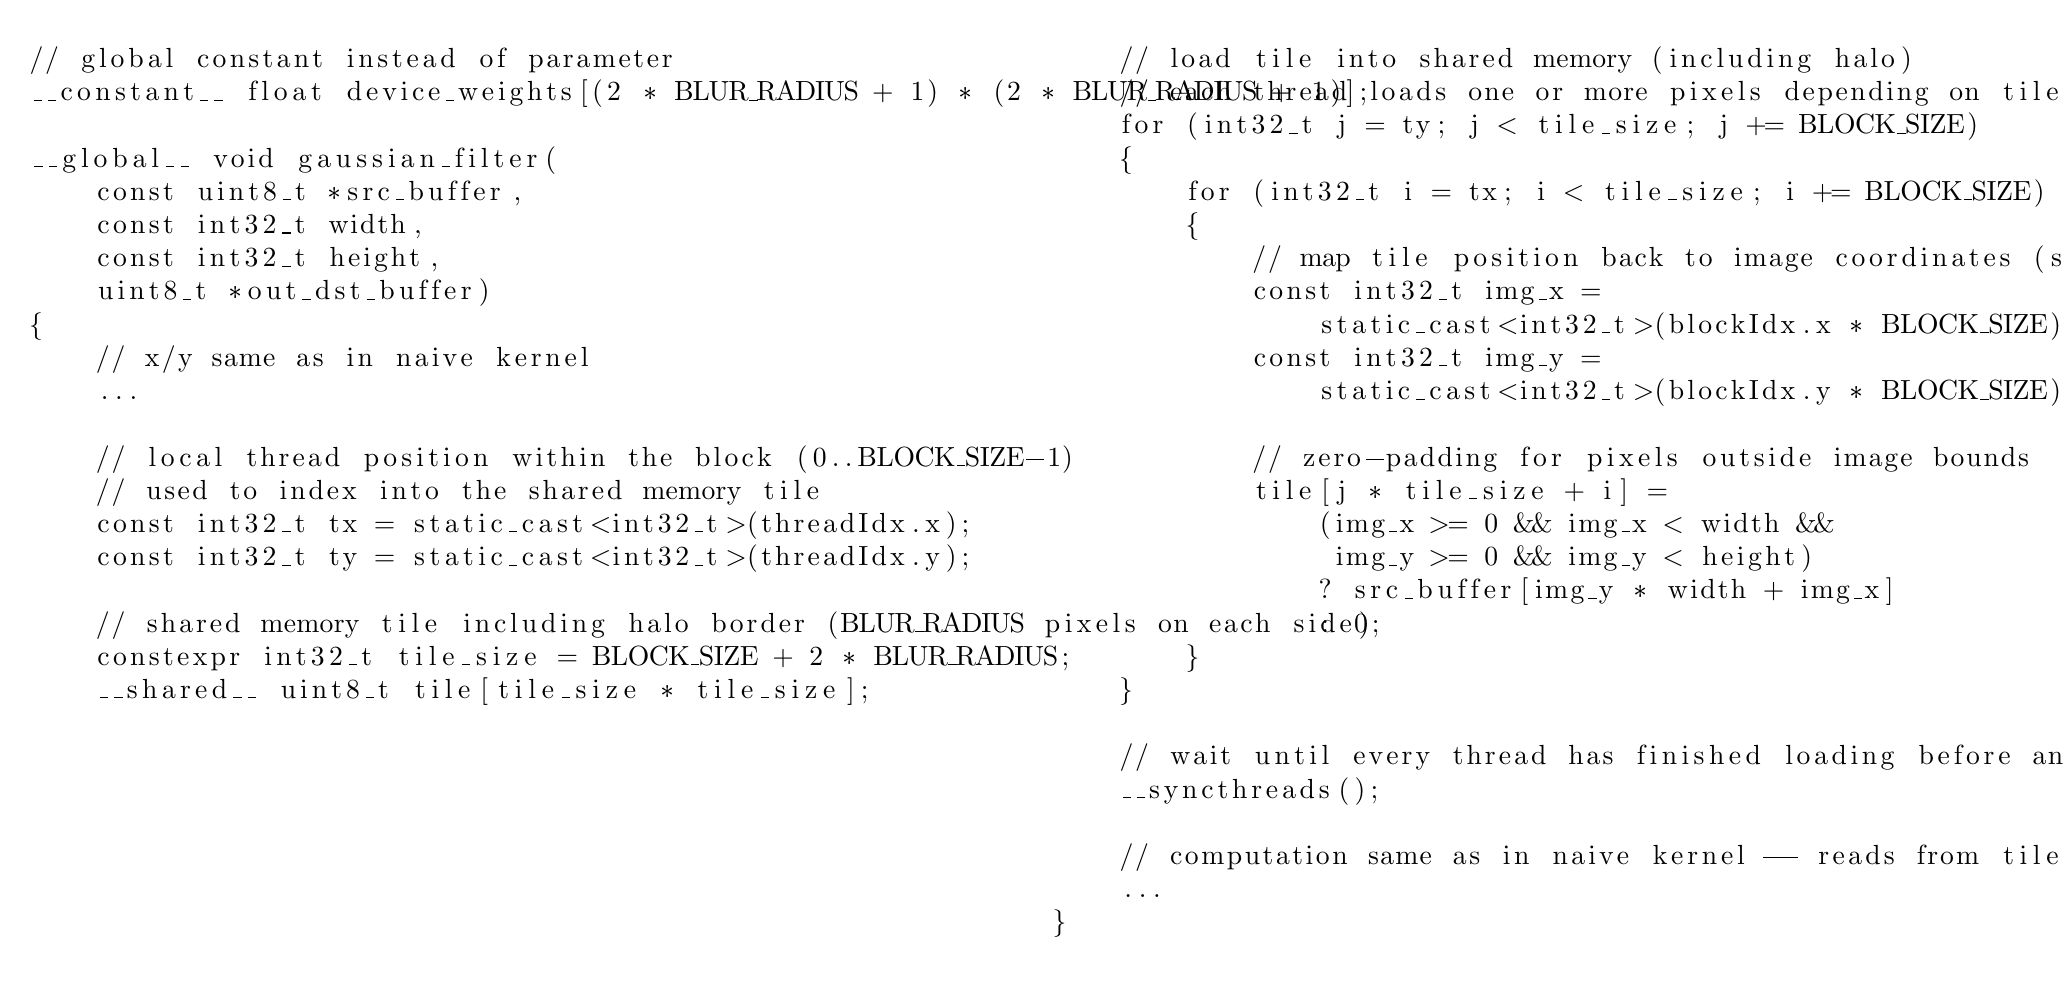
\begin{tikzpicture}[remember picture]

\node[inner sep=0pt, anchor=north west] (code) at (0,0) {%
    \begin{minipage}{12.5cm}
        \begin{lstlisting}
// global constant instead of parameter
__constant__ float device_weights[(2 * BLUR_RADIUS + 1) * (2 * BLUR_RADIUS + 1)];

__global__ void gaussian_filter(
    const uint8_t *src_buffer,
    const int32_t width,
    const int32_t height,
    uint8_t *out_dst_buffer)
{
    // x/y same as in naive kernel
    ...

    // local thread position within the block (0..BLOCK_SIZE-1)
    // used to index into the shared memory tile
    const int32_t tx = static_cast<int32_t>(threadIdx.x);
    const int32_t ty = static_cast<int32_t>(threadIdx.y);

    // shared memory tile including halo border (BLUR_RADIUS pixels on each side)
    constexpr int32_t tile_size = BLOCK_SIZE + 2 * BLUR_RADIUS;
    __shared__ uint8_t tile[tile_size * tile_size];
        \end{lstlisting}
    \end{minipage}%
};

\node[inner sep=0pt, anchor=north west] (code2) at (13.0,0) {%
    \begin{minipage}{12.5cm}
        \begin{lstlisting}[firstnumber=21]
    // load tile into shared memory (including halo)
    // each thread loads one or more pixels depending on tile size vs block size
    for (int32_t j = ty; j < tile_size; j += BLOCK_SIZE)
    {
        for (int32_t i = tx; i < tile_size; i += BLOCK_SIZE)
        {
            // map tile position back to image coordinates (subtract halo offset)
            const int32_t img_x =
                static_cast<int32_t>(blockIdx.x * BLOCK_SIZE) + i - BLUR_RADIUS;
            const int32_t img_y =
                static_cast<int32_t>(blockIdx.y * BLOCK_SIZE) + j - BLUR_RADIUS;

            // zero-padding for pixels outside image bounds
            tile[j * tile_size + i] =
                (img_x >= 0 && img_x < width &&
                 img_y >= 0 && img_y < height)
                ? src_buffer[img_y * width + img_x]
                : 0;
        }
    }

    // wait until every thread has finished loading before any thread starts reading
    __syncthreads();

    // computation same as in naive kernel -- reads from tile[] instead of src_buffer[]
    ...
}
        \end{lstlisting}
    \end{minipage}%
};

    \end{tikzpicture}
\end{document}